\begin{frame}[fragile]
  \begin{verbatim}
checker = InteractiveInvariantConfluenceChecker()
x = checker.int_max('x', 0) # An int, x, merged by max.
y = checker.int_max('y', 0) # An int, y, merged by max.
checker.add_transaction('inc_x', [x.assign(x + 1)])
checker.add_transaction('dec_y', [y.assign(y - 1)])
checker.add_invariant(x * y <= 0)
checker.check()\end{verbatim}
\end{frame}

\begin{frame}
  \begin{itemize}
    \item Foreign keys
    \item Auction application
    \item Escrow transactions
    \item TPC-C
  \end{itemize}

  \pause
  All run in less than a second and are implemented in less than 75 lines of
  specification.
\end{frame}

\begin{frame}
  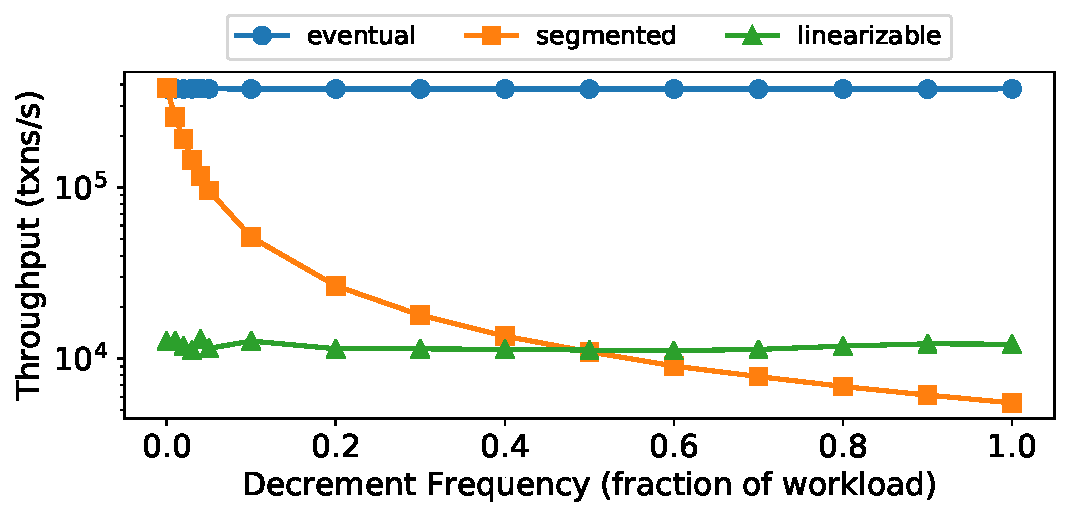
\includegraphics[width=\textwidth]{assets/throughput_vs_fraction_16.pdf}
\end{frame}

\begin{frame}
  \begin{center}
    \Huge
    Come to our poster tomorrow night!
  \end{center}
\end{frame}

\begin{frame}
  \begin{center}
    \Huge
    Thank you
  \end{center}
\end{frame}
